% Created by tikzDevice version 0.12 on 2019-04-28 00:12:43
% !TEX encoding = UTF-8 Unicode
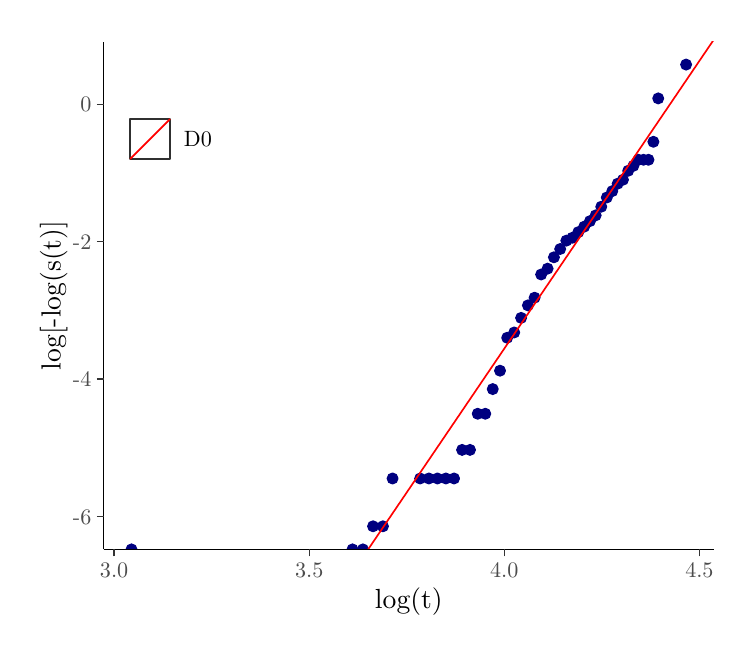
\begin{tikzpicture}[x=1pt,y=1pt]
\definecolor{fillColor}{RGB}{255,255,255}
\path[use as bounding box,fill=fillColor,fill opacity=0.00] (0,0) rectangle (252.94,216.81);
\begin{scope}
\path[clip] (  0.00,  0.00) rectangle (252.94,216.81);
\definecolor{drawColor}{RGB}{255,255,255}
\definecolor{fillColor}{RGB}{255,255,255}

\path[draw=drawColor,line width= 0.5pt,line join=round,line cap=round,fill=fillColor] ( -0.00,  0.00) rectangle (252.95,216.81);
\end{scope}
\begin{scope}
\path[clip] ( 27.50, 28.28) rectangle (247.95,211.81);
\definecolor{fillColor}{RGB}{255,255,255}

\path[fill=fillColor] ( 27.50, 28.28) rectangle (247.95,211.81);
\definecolor{drawColor}{RGB}{0,0,128}
\definecolor{fillColor}{RGB}{0,0,128}

\path[draw=drawColor,line width= 0.4pt,line join=round,line cap=round,fill=fillColor] ( 37.52, 28.28) circle (  1.96);

\path[draw=drawColor,line width= 0.4pt,line join=round,line cap=round,fill=fillColor] (117.38, 28.28) circle (  1.96);

\path[draw=drawColor,line width= 0.4pt,line join=round,line cap=round,fill=fillColor] (121.14, 28.28) circle (  1.96);

\path[draw=drawColor,line width= 0.4pt,line join=round,line cap=round,fill=fillColor] (124.80, 36.63) circle (  1.96);

\path[draw=drawColor,line width= 0.4pt,line join=round,line cap=round,fill=fillColor] (128.37, 36.63) circle (  1.96);

\path[draw=drawColor,line width= 0.4pt,line join=round,line cap=round,fill=fillColor] (131.85, 53.91) circle (  1.96);

\path[draw=drawColor,line width= 0.4pt,line join=round,line cap=round,fill=fillColor] (141.81, 53.91) circle (  1.96);

\path[draw=drawColor,line width= 0.4pt,line join=round,line cap=round,fill=fillColor] (144.97, 53.91) circle (  1.96);

\path[draw=drawColor,line width= 0.4pt,line join=round,line cap=round,fill=fillColor] (148.07, 53.91) circle (  1.96);

\path[draw=drawColor,line width= 0.4pt,line join=round,line cap=round,fill=fillColor] (151.11, 53.91) circle (  1.96);

\path[draw=drawColor,line width= 0.4pt,line join=round,line cap=round,fill=fillColor] (154.07, 53.91) circle (  1.96);

\path[draw=drawColor,line width= 0.4pt,line join=round,line cap=round,fill=fillColor] (156.98, 64.24) circle (  1.96);

\path[draw=drawColor,line width= 0.4pt,line join=round,line cap=round,fill=fillColor] (159.83, 64.24) circle (  1.96);

\path[draw=drawColor,line width= 0.4pt,line join=round,line cap=round,fill=fillColor] (162.62, 77.30) circle (  1.96);

\path[draw=drawColor,line width= 0.4pt,line join=round,line cap=round,fill=fillColor] (165.36, 77.30) circle (  1.96);

\path[draw=drawColor,line width= 0.4pt,line join=round,line cap=round,fill=fillColor] (168.05, 86.21) circle (  1.96);

\path[draw=drawColor,line width= 0.4pt,line join=round,line cap=round,fill=fillColor] (170.68, 92.86) circle (  1.96);

\path[draw=drawColor,line width= 0.4pt,line join=round,line cap=round,fill=fillColor] (173.27,104.76) circle (  1.96);

\path[draw=drawColor,line width= 0.4pt,line join=round,line cap=round,fill=fillColor] (175.81,106.67) circle (  1.96);

\path[draw=drawColor,line width= 0.4pt,line join=round,line cap=round,fill=fillColor] (178.30,111.94) circle (  1.96);

\path[draw=drawColor,line width= 0.4pt,line join=round,line cap=round,fill=fillColor] (180.76,116.46) circle (  1.96);

\path[draw=drawColor,line width= 0.4pt,line join=round,line cap=round,fill=fillColor] (183.17,119.23) circle (  1.96);

\path[draw=drawColor,line width= 0.4pt,line join=round,line cap=round,fill=fillColor] (185.54,127.62) circle (  1.96);

\path[draw=drawColor,line width= 0.4pt,line join=round,line cap=round,fill=fillColor] (187.87,129.73) circle (  1.96);

\path[draw=drawColor,line width= 0.4pt,line join=round,line cap=round,fill=fillColor] (190.16,133.83) circle (  1.96);

\path[draw=drawColor,line width= 0.4pt,line join=round,line cap=round,fill=fillColor] (192.42,136.83) circle (  1.96);

\path[draw=drawColor,line width= 0.4pt,line join=round,line cap=round,fill=fillColor] (194.64,139.85) circle (  1.96);

\path[draw=drawColor,line width= 0.4pt,line join=round,line cap=round,fill=fillColor] (196.82,140.89) circle (  1.96);

\path[draw=drawColor,line width= 0.4pt,line join=round,line cap=round,fill=fillColor] (198.97,142.92) circle (  1.96);

\path[draw=drawColor,line width= 0.4pt,line join=round,line cap=round,fill=fillColor] (201.09,144.90) circle (  1.96);

\path[draw=drawColor,line width= 0.4pt,line join=round,line cap=round,fill=fillColor] (203.18,146.91) circle (  1.96);

\path[draw=drawColor,line width= 0.4pt,line join=round,line cap=round,fill=fillColor] (205.24,148.98) circle (  1.96);

\path[draw=drawColor,line width= 0.4pt,line join=round,line cap=round,fill=fillColor] (207.27,152.11) circle (  1.96);

\path[draw=drawColor,line width= 0.4pt,line join=round,line cap=round,fill=fillColor] (209.27,155.44) circle (  1.96);

\path[draw=drawColor,line width= 0.4pt,line join=round,line cap=round,fill=fillColor] (211.24,157.74) circle (  1.96);

\path[draw=drawColor,line width= 0.4pt,line join=round,line cap=round,fill=fillColor] (213.19,160.43) circle (  1.96);

\path[draw=drawColor,line width= 0.4pt,line join=round,line cap=round,fill=fillColor] (215.11,161.86) circle (  1.96);

\path[draw=drawColor,line width= 0.4pt,line join=round,line cap=round,fill=fillColor] (217.00,165.10) circle (  1.96);

\path[draw=drawColor,line width= 0.4pt,line join=round,line cap=round,fill=fillColor] (218.87,166.87) circle (  1.96);

\path[draw=drawColor,line width= 0.4pt,line join=round,line cap=round,fill=fillColor] (220.71,169.07) circle (  1.96);

\path[draw=drawColor,line width= 0.4pt,line join=round,line cap=round,fill=fillColor] (222.53,169.07) circle (  1.96);

\path[draw=drawColor,line width= 0.4pt,line join=round,line cap=round,fill=fillColor] (224.32,169.07) circle (  1.96);

\path[draw=drawColor,line width= 0.4pt,line join=round,line cap=round,fill=fillColor] (226.10,175.57) circle (  1.96);

\path[draw=drawColor,line width= 0.4pt,line join=round,line cap=round,fill=fillColor] (227.85,191.25) circle (  1.96);

\path[draw=drawColor,line width= 0.4pt,line join=round,line cap=round,fill=fillColor] (237.92,203.47) circle (  1.96);
\definecolor{drawColor}{RGB}{255,0,0}

\path[draw=drawColor,line width= 0.6pt,line join=round] (103.84,  0.00) -- (247.95,212.51);
\end{scope}
\begin{scope}
\path[clip] (  0.00,  0.00) rectangle (252.94,216.81);
\definecolor{drawColor}{RGB}{0,0,0}

\path[draw=drawColor,line width= 0.5pt,line join=round] ( 27.50, 28.28) --
	( 27.50,211.81);
\end{scope}
\begin{scope}
\path[clip] (  0.00,  0.00) rectangle (252.94,216.81);
\definecolor{drawColor}{gray}{0.30}

\node[text=drawColor,anchor=base east,inner sep=0pt, outer sep=0pt, scale=  0.80] at ( 23.00, 37.42) {-6};

\node[text=drawColor,anchor=base east,inner sep=0pt, outer sep=0pt, scale=  0.80] at ( 23.00, 87.07) {-4};

\node[text=drawColor,anchor=base east,inner sep=0pt, outer sep=0pt, scale=  0.80] at ( 23.00,136.71) {-2};

\node[text=drawColor,anchor=base east,inner sep=0pt, outer sep=0pt, scale=  0.80] at ( 23.00,186.35) {0};
\end{scope}
\begin{scope}
\path[clip] (  0.00,  0.00) rectangle (252.94,216.81);
\definecolor{drawColor}{gray}{0.20}

\path[draw=drawColor,line width= 0.5pt,line join=round] ( 25.00, 40.18) --
	( 27.50, 40.18);

\path[draw=drawColor,line width= 0.5pt,line join=round] ( 25.00, 89.82) --
	( 27.50, 89.82);

\path[draw=drawColor,line width= 0.5pt,line join=round] ( 25.00,139.46) --
	( 27.50,139.46);

\path[draw=drawColor,line width= 0.5pt,line join=round] ( 25.00,189.11) --
	( 27.50,189.11);
\end{scope}
\begin{scope}
\path[clip] (  0.00,  0.00) rectangle (252.94,216.81);
\definecolor{drawColor}{RGB}{0,0,0}

\path[draw=drawColor,line width= 0.5pt,line join=round] ( 27.50, 28.28) --
	(247.95, 28.28);
\end{scope}
\begin{scope}
\path[clip] (  0.00,  0.00) rectangle (252.94,216.81);
\definecolor{drawColor}{gray}{0.20}

\path[draw=drawColor,line width= 0.5pt,line join=round] ( 31.24, 25.78) --
	( 31.24, 28.28);

\path[draw=drawColor,line width= 0.5pt,line join=round] (101.74, 25.78) --
	(101.74, 28.28);

\path[draw=drawColor,line width= 0.5pt,line join=round] (172.23, 25.78) --
	(172.23, 28.28);

\path[draw=drawColor,line width= 0.5pt,line join=round] (242.73, 25.78) --
	(242.73, 28.28);
\end{scope}
\begin{scope}
\path[clip] (  0.00,  0.00) rectangle (252.94,216.81);
\definecolor{drawColor}{gray}{0.30}

\node[text=drawColor,anchor=base,inner sep=0pt, outer sep=0pt, scale=  0.80] at ( 31.24, 18.28) {3.0};

\node[text=drawColor,anchor=base,inner sep=0pt, outer sep=0pt, scale=  0.80] at (101.74, 18.28) {3.5};

\node[text=drawColor,anchor=base,inner sep=0pt, outer sep=0pt, scale=  0.80] at (172.23, 18.28) {4.0};

\node[text=drawColor,anchor=base,inner sep=0pt, outer sep=0pt, scale=  0.80] at (242.73, 18.28) {4.5};
\end{scope}
\begin{scope}
\path[clip] (  0.00,  0.00) rectangle (252.94,216.81);
\definecolor{drawColor}{RGB}{0,0,0}

\node[text=drawColor,anchor=base,inner sep=0pt, outer sep=0pt, scale=  1.00] at (137.72,  6.94) {log(t)};
\end{scope}
\begin{scope}
\path[clip] (  0.00,  0.00) rectangle (252.94,216.81);
\definecolor{drawColor}{RGB}{0,0,0}

\node[text=drawColor,rotate= 90.00,anchor=base,inner sep=0pt, outer sep=0pt, scale=  1.00] at ( 11.89,120.05) {log[-log(s(t)]};
\end{scope}
\begin{scope}
\path[clip] (  0.00,  0.00) rectangle (252.94,216.81);
\definecolor{fillColor}{RGB}{255,255,255}

\path[fill=fillColor] ( 32.02,164.35) rectangle ( 71.59,202.63);
\end{scope}
\begin{scope}
\path[clip] (  0.00,  0.00) rectangle (252.94,216.81);
\definecolor{drawColor}{RGB}{0,0,0}

\node[text=drawColor,anchor=base west,inner sep=0pt, outer sep=0pt, scale=  1.00] at ( 37.02,189.77) { };
\end{scope}
\begin{scope}
\path[clip] (  0.00,  0.00) rectangle (252.94,216.81);
\definecolor{drawColor}{gray}{0.19}
\definecolor{fillColor}{RGB}{255,255,255}

\path[draw=drawColor,line width= 0.5pt,line join=round,line cap=round,fill=fillColor] ( 37.02,169.35) rectangle ( 51.48,183.80);
\end{scope}
\begin{scope}
\path[clip] (  0.00,  0.00) rectangle (252.94,216.81);
\definecolor{drawColor}{RGB}{255,0,0}

\path[draw=drawColor,line width= 0.6pt,line join=round] ( 37.02,169.35) -- ( 51.48,183.80);
\end{scope}
\begin{scope}
\path[clip] (  0.00,  0.00) rectangle (252.94,216.81);
\definecolor{drawColor}{RGB}{0,0,0}

\node[text=drawColor,anchor=base west,inner sep=0pt, outer sep=0pt, scale=  0.80] at ( 56.48,173.82) {D0};
\end{scope}
\end{tikzpicture}
